\documentclass[8pt,a4paper,compress]{beamer}

\usepackage{/home/siyer/lib/slides}

\title{Directed Graphs}
\date{}
\begin{document}
\begin{frame}
\vfill
\titlepage
\end{frame}

\begin{frame}
\frametitle{Outline}
\tableofcontents
\end{frame}

\section{Directed Graphs}
\begin{frame}[fragile]
\begin{minipage}{200pt}
\begin{itemize}
\item a directed graph (digraph) is a set of vertices and a collection of directed edges, each connecting an ordered pair of vertices

\item the outdegree of a vertex in a digraph is the number of edges
going from it; the indegree of a vertex is the number of edges going to it

\item a directed path in a digraph is a sequence of vertices in which there is a (directed) edge pointing from each vertex in the sequence to its successor in the sequence

\item a directed cycle is a directed path with at least one edge whose first and last vertices are the same

\item the length of a path or a cycle is its number of edges
\end{itemize}
\end{minipage}%
\begin{minipage}{100pt}
\begin{center}
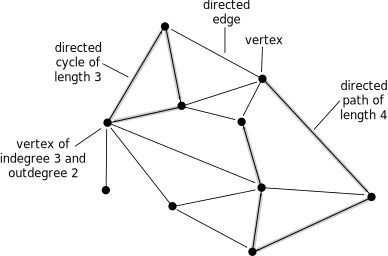
\includegraphics[scale=0.45]{{./figures/digraph1}.png}

\tiny anatomy of a digraph
\end{center}
\end{minipage}
\end{frame}

\begin{frame}[fragile]
\begin{itemize}
\item digraph applications
\begin{center}
\begin{tabular}{ccc}
\textbf{digraph} & \textbf{vertex} & \textbf{edge} \\ \hline \\
transportation & street intersection & one-way street \\
web & web page & hyperlink \\
food web & species & predator-prey relationship \\
WordNet & synset & hypernym \\
scheduling & task & precedence constraint \\
financial & bank & transaction \\
cell phone & person & placed call \\
infectious disease & person & infection \\
game & board position & legal move \\
citation & journal article & citation \\
object graph & object & pointer \\
inheritance hierarchy & class & inherits from \\ 
control flow & code block & jump
\end{tabular}  
\end{center}
\end{itemize}
\end{frame}

\begin{frame}[fragile]
\begin{itemize}
\item some digraph problems
\begin{center}
\begin{tabular}{cp{5cm}}
\textbf{problem} & \textbf{description} \\ \hline \\
$s\to t$ path & is there a path from $s$ to $t$? \\ 
shortest $s\to t$ path & what is the shortest path from $s$ to $t$? \\
directed cycle & is there a directed cycle in the graph? \\
topological sort & can the digraph be drawn so that all edges point in a single direction? \\
strong connectivity & is there a directed path between all pairs of vertices? \\
transitive closure & for which vertices $v$ and $w$ is there a directed path from $v$ to $w$? \\
PageRank & what is the importance of a web page?
\end{tabular}  
\end{center}
\end{itemize}
\end{frame}

\begin{frame}[fragile]
\begin{itemize}
\item digraph API
\begin{lstlisting}[language={},mathescape]
public class Digraph

    Digraph(int V) // create an empty digraph with $V$ vertices
    Digraph(In in) // create a digraph from input stream
    void addEdge(int v, int w)   // add a directed edge $v \to w$
    Iterable<Integer> adj(int v) // vertices pointing from $v$
    int V()                      // number of vertices
    int E()                      // number of edges
    Digraph reverse()            // reverse of this digraph
\end{lstlisting}

\item graph input format
\begin{minipage}{150pt}
\begin{lstlisting}[language={}]
$ more tinyG.txt
13 22
 4 2
 2 3
 3 2
 6 0
 0 1
 2 0
11 12
12 9
...
\end{lstlisting}
\end{minipage}%
\begin{minipage}{150pt}
\begin{center}
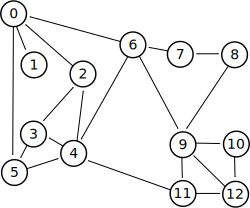
\includegraphics[scale=0.5]{{./figures/digraph2}.png}
\end{center}
\end{minipage}

\item typical graph-processing code
\begin{lstlisting}[language=Java]
In in = new In(args[0]);
Digraph G = new Digraph(in);
for (int v = 0; v < G.V(); v++) {
    for (int w : G.adj(v)) {
        StdOut.println(v + "->" + w);
    }
}
\end{lstlisting}
\end{itemize}
\end{frame}

\begin{frame}[fragile]
\begin{itemize}
\item digraph implementation
\begin{lstlisting}[language=Java]
public class Digraph {
    private final int V;
    private int E;
    private LinkedBag<Integer>[] adj;

    public Digraph(int V) {
        if (V < 0) { throw new IllegalArgumentException(...); }
        this.V = V;
        this.E = 0;
        adj = (LinkedBag<Integer>[]) new LinkedBag[V];
        for (int v = 0; v < V; v++) {
            adj[v] = new LinkedBag<Integer>();
        }
    }

    public Digraph(In in) {
        this.V = in.readInt();
        if (V < 0) { throw new IllegalArgumentException(...); }
        adj = (LinkedBag<Integer>[]) new LinkedBag[V];
        for (int v = 0; v < V; v++) {
            adj[v] = new LinkedBag<Integer>();
        }
        int E = in.readInt();
        if (E < 0) { throw new IllegalArgumentException(...); }
        for (int i = 0; i < E; i++) {
            int v = in.readInt();
            int w = in.readInt();
            addEdge(v, w); 
        }
    }
    ...
}
\end{lstlisting}
\end{itemize}
\end{frame}

\begin{frame}[fragile]
\begin{itemize}
\item digraph implementation (contd.)
\begin{lstlisting}[language=Java]
public class Digraph {
    ...
    public int V() { return V; }

    public int E() { return E; }

    private void validateVertex(int v) {
        if (v < 0 || v >= V) { throw new IndexOutOfBoundsException(...); }
    }

    public void addEdge(int v, int w) {
        validateVertex(v);
        validateVertex(w);
        adj[v].add(w);
        E++;
    }

    public Iterable<Integer> adj(int v) {
        validateVertex(v);
        return adj[v];
    }

    public Digraph reverse() {
        Digraph R = new Digraph(V);
        for (int v = 0; v < V; v++) {
            for (int w : adj(v)) {
                R.addEdge(w, v);
            }
        }
        return R;
    }
    ...
}
\end{lstlisting}
\end{itemize}
\end{frame}

\section{Depth-First Search (DFS)}
\begin{frame}[fragile]
\begin{itemize}
\item same method as for undirected graphs, ie, to visit a vertex $v$
\begin{itemize}
\item mark a vertex $v$ as visited

\item recursively visit all unmarked vertices pointing from $v$
\end{itemize}

\item reachability problem
\begin{itemize}
\item single-source reachability: given a digraph and a source vertex $s$, support queries of the form \emph{is there a directed path from $s$ to a given target vertex $v$?}

\item multi-source reachability: given a digraph and a set of source vertices, support queries of the form \emph{is there a directed path from any vertex in the set to a given target vertex $v$?}
\end{itemize}

\item applications
\begin{itemize}
\item program control-flow analysis such as dead-code elimination and  infinite-loop detection

\item mark and sweep garbage collector
\end{itemize}
\end{itemize}
\end{frame}

\section{Breadth-First Search (BFS)}
\begin{frame}[fragile]
\begin{itemize}
\item same method as for undirected graphs, ie, repeat until queue is empty
\begin{itemize}
\item remove vertex $v$ from queue

\item add to queue all unmarked vertices pointing from $v$ and mark them
\end{itemize}

\item BFS computes shortest paths (fewest number of edges)
from source vertex $s$ to all other vertices in a digraph in time proportional to $E + V$

\item multiple-source shortest paths: given a digraph and a set of source vertices, find shortest path from any vertex in the set to each other vertex; solution: use BFS, but initialize by enqueuing all source vertices
\end{itemize}
\end{frame}

\begin{frame}[fragile]
\begin{itemize}
\item application: web crawler
\begin{lstlisting}[language=Java]
public class WebCrawler { 
    public static void main(String[] args) { 
        String s = args[0];
        LinkedQueue<String> queue = new LinkedQueue<String>();
        queue.enqueue(s);
        OrderedSet<String> marked = new OrderedSet<String>();
        marked.add(s);
        while (!queue.isEmpty()) {
            String v = queue.dequeue();
            System.out.println(v);
            In in = new In(v);
            if (!in.exists()) { continue; }
            String input = in.readAll();
            if (input == null) { continue; }
            String regexp = "http://(\\w+\\.)+(\\w+)";
            Pattern pattern = Pattern.compile(regexp);
            Matcher matcher = pattern.matcher(input);
            while (matcher.find()) {
                String w = matcher.group();
                if (!marked.contains(w)) {
                    queue.enqueue(w);
                    marked.add(w);
                }
            }
        }
    }
}
\end{lstlisting}

\begin{lstlisting}[language={}]
$ java WebCrawler http://www.swamiiyer.net/
http://www.swamiiyer.net/
http://www.w3.org
http://jemdoc.jaboc.net
...
\end{lstlisting}
\end{itemize}
\end{frame}

\section{Topological Sort}
\begin{frame}[fragile]
\begin{itemize}
\item precedence-constrained scheduling: given a set of jobs to be completed, with precedence constraints that specify that certain jobs have to be completed before certain other jobs are begun, how can we schedule the jobs such that they are all completed while still respecting the constraints?

\begin{center}
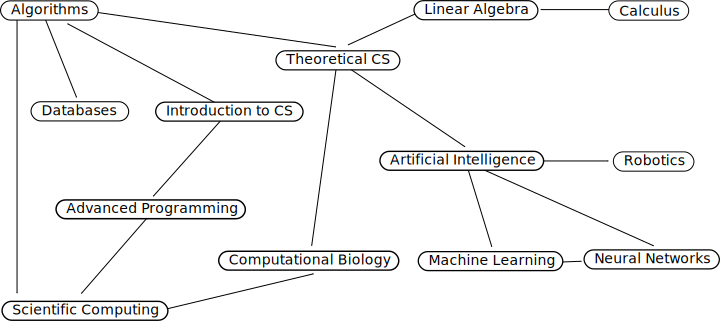
\includegraphics[scale=0.4]{{./figures/digraph3}.png}

\smallskip

\small a precedence-constrained scheduling problem

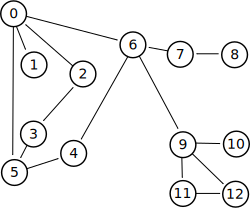
\includegraphics[scale=0.4]{{./figures/digraph4}.png}

\smallskip

\small standard digraph model
\end{center}


\end{itemize}
\end{frame}

\begin{frame}[fragile]
\begin{itemize}
\item topological sort: given a DAG (a directed acyclic graph), put the vertices in order such that all its directed edges point from a vertex earlier in the order to a vertex later in the order

\begin{center}
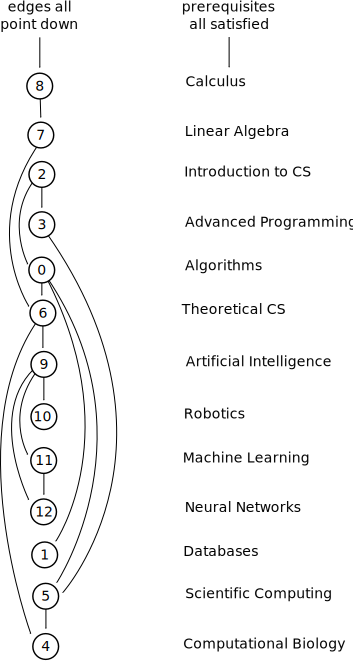
\includegraphics[scale=0.35]{{./figures/digraph5}.png}
\end{center}

\item a digraph has a topological order if and only if it is a DAG
\end{itemize}
\end{frame}

\begin{frame}[fragile]
\begin{itemize}
\item directed cycle detection (see \lstinline{DirectedCycle}) applications
\begin{itemize}
\item cyclic inheritance

\item circular references in spreadsheet calculations
\end{itemize}

\item depth-first search orders (see \lstinline{DepthFirstOrder})
\begin{itemize}
\item preorder: order in which \lstinline{dfs()} is called

\item postorder: order in which \lstinline{dfs()} returns

\item reverse postorder: reverse order in which \lstinline{dfs()} returns
\end{itemize}

\begin{lstlisting}[language=Java]
private void dfs(Graph G, int v) {
    marked[v] = true;
    preorder.enqueue(v);
    for (int w : G.adj(v)) {
        if (!marked[w]) { dfs(G, w); }
    }
    postorder.enqueue(v);
    reversePostorder.push(v);
}
\end{lstlisting}
\end{itemize}
\end{frame}

\begin{frame}[fragile]
\begin{itemize}
\item topological sort: solution

\begin{itemize}
\item run depth-first search

\item return vertices in reverse postorder
\end{itemize}

\item topological sort: implementation
\begin{lstlisting}[language=Java]
public class Topological {
    private Iterable<Integer> order; 

    public Topological(Digraph G) {
        DirectedCycle finder = new DirectedCycle(G);
        if (!finder.hasCycle()) {
            DepthFirstOrder dfs = new DepthFirstOrder(G);
            order = dfs.reversePost();
        }
    }
    
    public Iterable<Integer> order() { return order; }

    public boolean hasOrder() { return order != null; }

    ...
}
\end{lstlisting}
\end{itemize}
\end{frame}

\section{Strong Components}
\begin{frame}[fragile]
\begin{itemize}
\item vertices $v$ and $w$ are strongly connected if there is both a directed path from $v$ to $w$ and a directed path from $w$ to $v$

\begin{center}
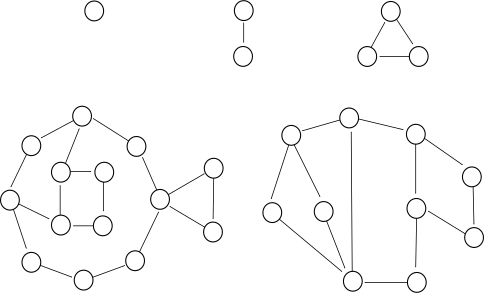
\includegraphics[scale=0.35]{{./figures/digraph6}.png}

\smallskip

\small strongly connected digraphs
\end{center}

\item a strong component is a maximal subset of strongly-connected vertices

\begin{center}
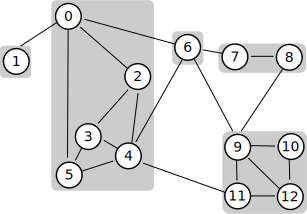
\includegraphics[scale=0.35]{{./figures/digraph7}.png}

\smallskip

\small a digraph and its strong components
\end{center}

\item applications
\begin{itemize}
\item ecological food web

\item software module dependency
\end{itemize}
\end{itemize}
\end{frame}

\begin{frame}[fragile]
\begin{itemize}
\item computing strong components: solution (Kosaraju-Sharir algorithm)
\begin{itemize}
\item given a digraph $G$, use \lstinline{DepthFirstOrder} to compute the reverse postorder of its reverse, $G^R$

\item run standard DFS on $G$, but consider the unmarked vertices in the order just computed instead of the standard numerical order

\item all vertices reached on a call to the recursive \lstinline{dfs()} from the constructor are in a strong component, so identify them as in \lstinline{CC}
\end{itemize}

\item Kosaraju-Sharir algorithm: implementation
\begin{lstlisting}[language=Java]
public class KosarajuSharirSCC {
    ...
    public KosarajuSharirSCC(Digraph G) {
        DepthFirstOrder dfs = new DepthFirstOrder(G.reverse());
        marked = new boolean[G.V()];
        id = new int[G.V()];
        for (int v : dfs.reversePost()) {
            if (!marked[v]) {
                dfs(G, v);
                count++;
            }
        }
    }
    
    private void dfs(Digraph G, int v) { 
        marked[v] = true;
        id[v] = count;
        for (int w : G.adj(v)) {
            if (!marked[w]) { dfs(G, w); }
        }
    }
    ...
}
\end{lstlisting}
\end{itemize}
\end{frame}
\end{document}
